\begin{figure}[!Ht]
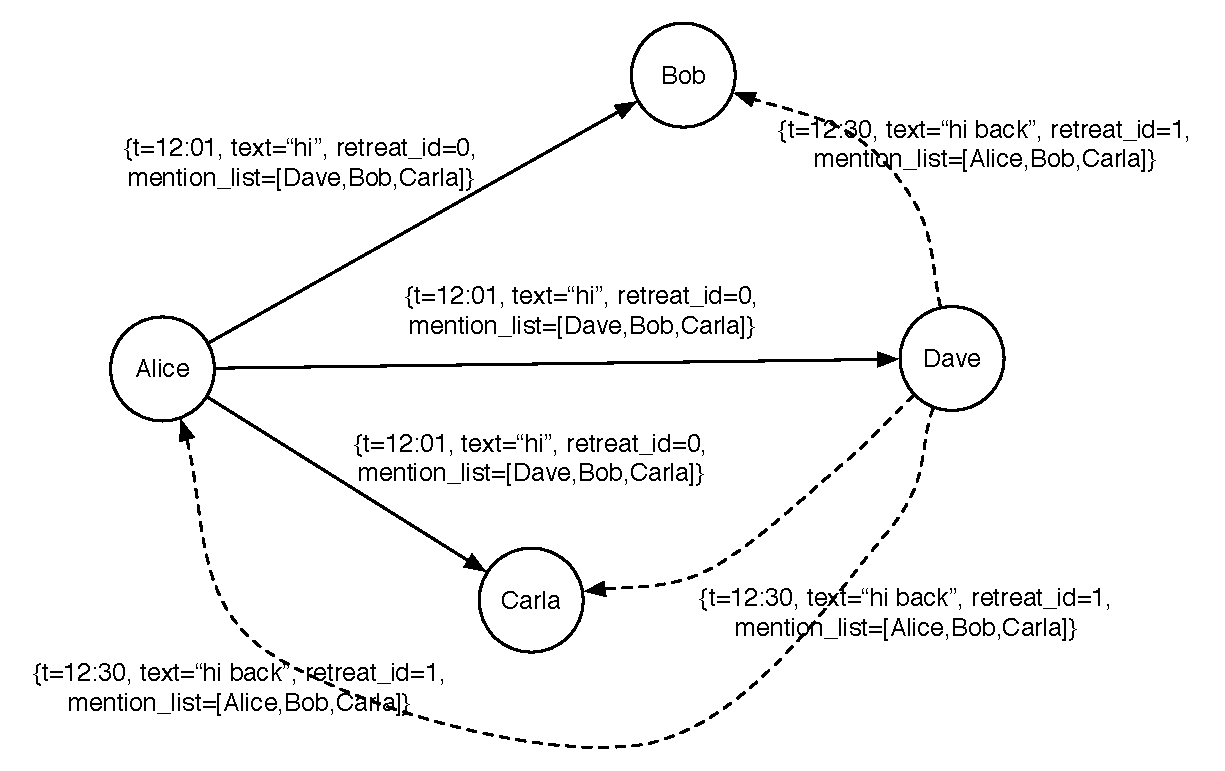
\includegraphics[width=0.9\columnwidth]{figures/example_interaction.pdf} 
 \caption{An example interaction graph for call data records, capturing the
   telephone call interactions among four people. Each edge in the graph is
   associated with attributes for the interaction, including the time the call
   was placed, the duration of the call, the cell phone tower, and the IMEI
   number identifying the device used.}
 \label{fig:example}
 \end{figure}


\section{System Overview}\label{sec:system}


The design of the railway disk layout builds on our prior work~\cite{gedik14}, 
which organized the disk layout for an interaction graph databases to improve
access locality. The railway layout extends the previous design, by enabling the
system to adapt the layout to reduce query I/O for changing workloads.

\paragraph*{Motivating Example}
%
To explain the design of the railway layout, we first introduce a small,
motivating example. Figure~\ref{fig:example} shows a graph for the telephone
call interactions among four people. This is a subset of the information that is
captured for call data records. Each edge in the graph is associated with
attributes for the interaction, including the time the call was placed, the
duration of the call, the cell phone tower, and the IMEI number identifying the
device used to place the call. In this example, there were four calls
placed. One of them was a call from Alice to Bob, starting at 13:46. They spoke
for 600 seconds. The call was received by cell phone tower 1, and the Alice's
phone had an IMEI number of 100.

A telecommunications company typically performs various analytics on this
data. For example, in order to understand how they should price their service
plans, they might want to capture the duration of all calls for each user. To
plan for infrastructure provisioning, they might want to record a count of the
number of calls that each cell phone tower handled.




\begin{figure*}[ht]
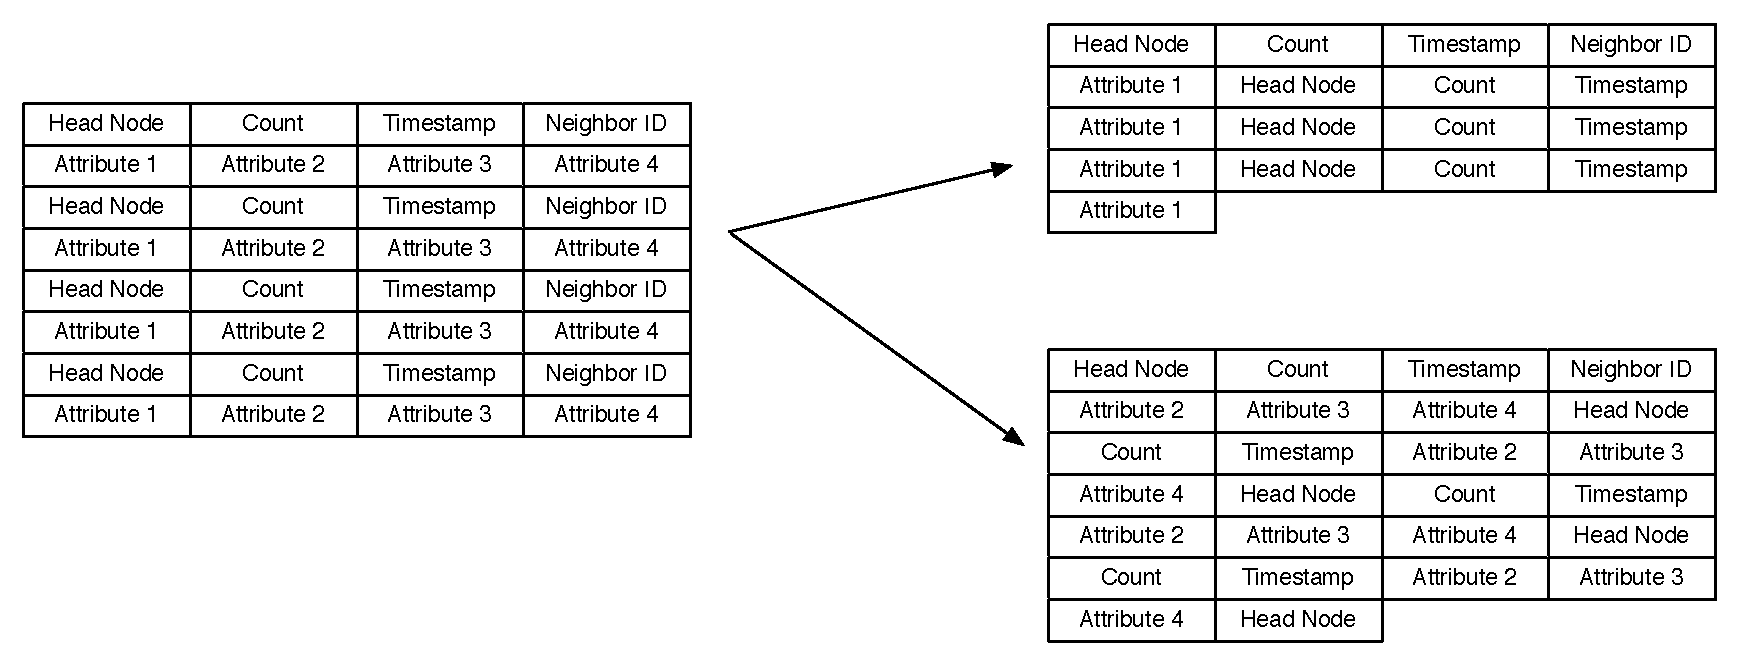
\includegraphics[width=0.9\textwidth]{figures/before_after.pdf} 
 \caption{The standard disk block strorage for an interaction graph, and a
   partitioning into sub-blocks for the railway layout. Each sub-block maintains
 its own copy of the neighbor list, but a subset of the attributes.}
 \label{fig:before_after}
 \end{figure*}

\paragraph*{Storage for Locality}
%
There are several ways in which one might store an interaction graph on
disk. The graph structure can be stored as a matrix representation or an
adjacency list. Most graph databases choose an adjacency list representation
because they reduce the storage overhead when graphs are sparse, and it is
faster to iterate over the edges when traversing the graph.  Attributes
associates with each edge could be stored in separately in a relational table,
or along with the edges. Storing the attributes with the edges improves the
locality, since the database can read the graph structure and associated
attributes from the same disk block. \rjs{Talk about timestamps.}


The lefthand side of Figure~\ref{fig:before_after} illustrates a disk layout
design with an adjacency list representation in which attributes are stored with
the edges. This is the design used in our prior work~\cite{gedik14}.


 typical storage for interaction graphs.
Each disk block contains an adjacency list representation of the interaction
graph. The block contains a sequence of vertices, identified by a
\emph{head-node id}, followed by a \emph{count} of the number of neighbors, and
then the neighbor list itself. Each entry in the neighbor list is composed of a
\emph{timestamp}, an \emph{id} for the destination vertex, and the properties
for that edge. 




\paragraph*{Rail Layout}
%




\begin{alltt}\scriptsize
- System overview
    - How interaction graph are currently stored
        - Most of the disk space work is on regular graphs, 
           not interaction graphs. 
        - Approach this as this is the railway, and we built
           on this prior work.
        - Builds on existing work that does not support 
          adaptivity.
    - Introduce the rail layout
    - Add the Figure~\ref{fig:rail_layout}
    - Query model
   - Note that we need to talk here:
    - For the system implementation, we need to add an additional
       index to have a list of partitions for a block
   - We also need to know how attributes are partitioned across sub-blocks 
      for a given time interval.

    - Current layout:
    head vertex (id), num items in neighbor list, 
    for each entry:
        timestamp of edge
        id of other edge of vertex
        any edge properties

\end{alltt}

\begin{figure}[ht]
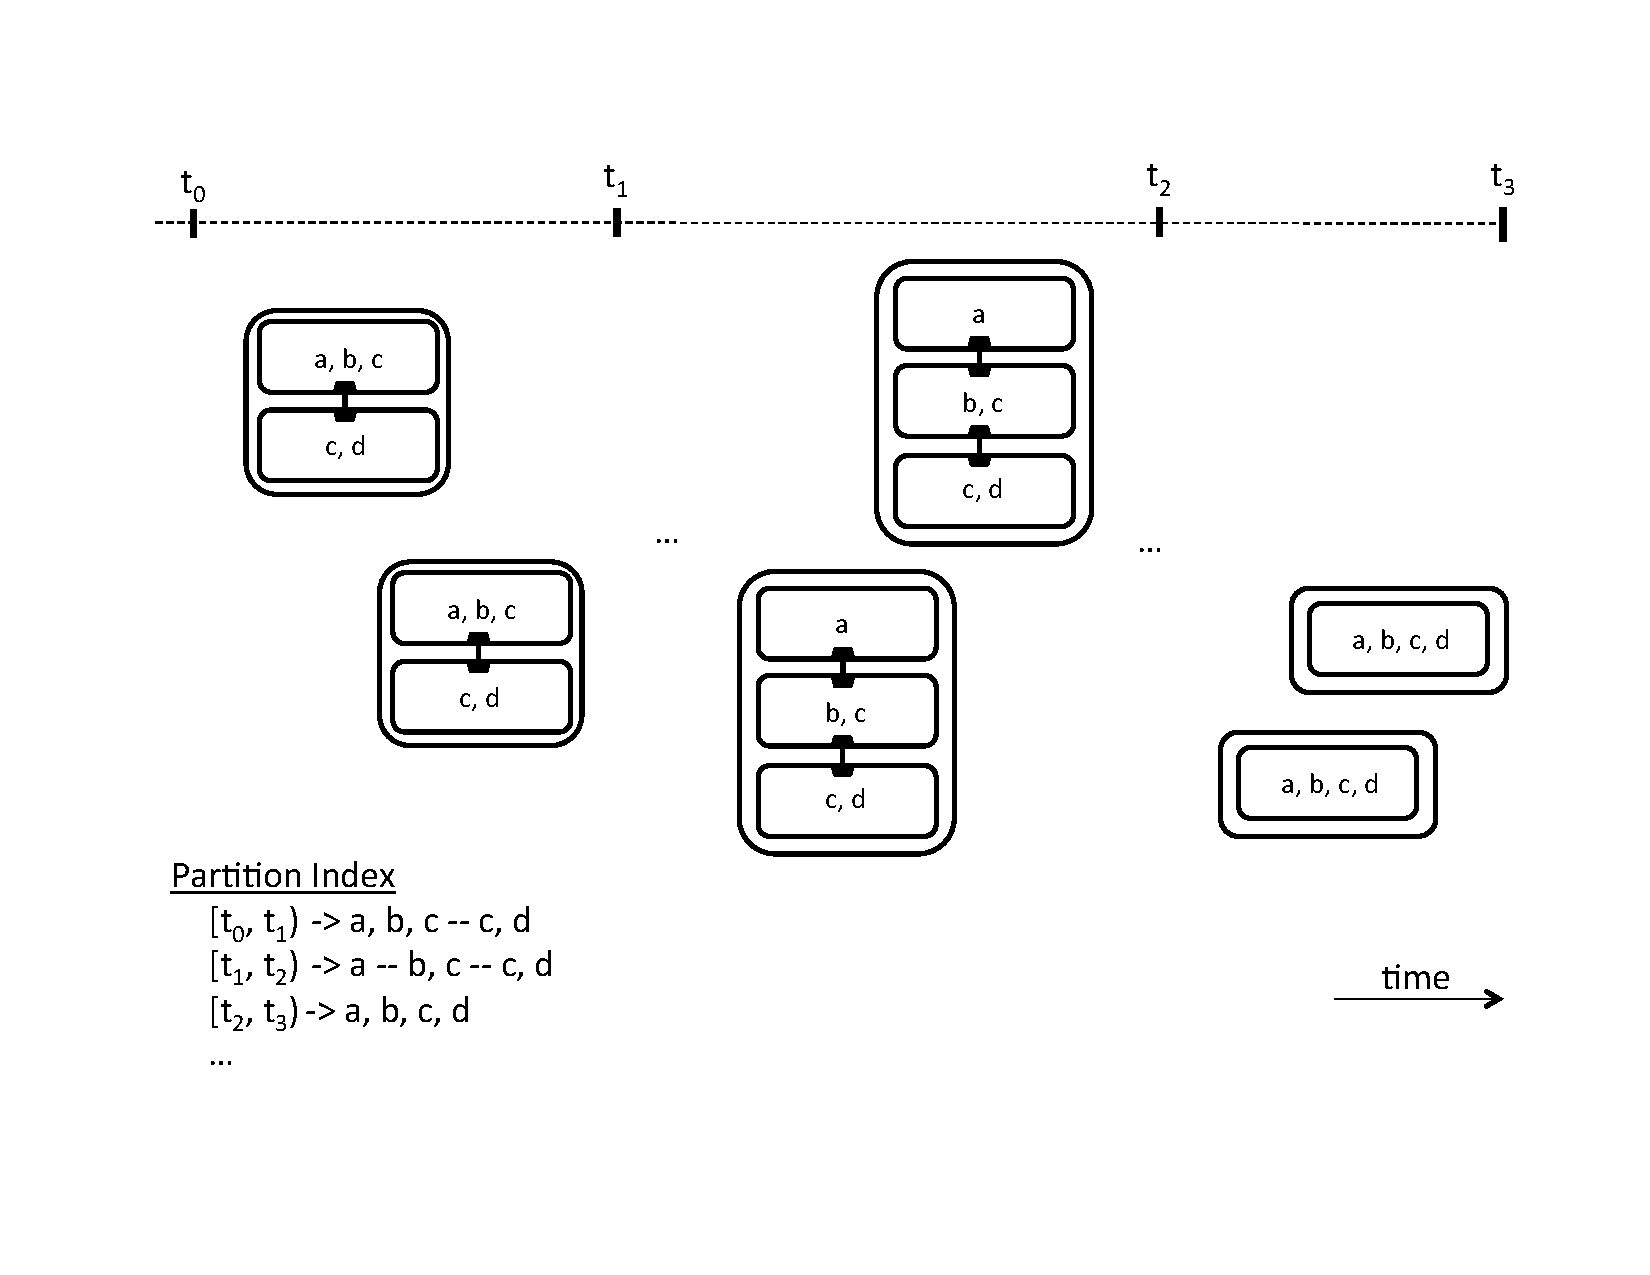
\includegraphics[width=0.9\columnwidth]{figures/rail_layout.pdf} 
 \caption{todo}
 \label{fig:rail_layout}
 \end{figure}
